\documentclass[12pt,utf8,notheorems,compress,t]{beamer}
\usepackage{etex}

\usepackage{pgfpages}
\usepackage[export]{adjustbox}
%\setbeameroption{show notes on second screen}
%\setbeamertemplate{note page}[plain]
%\newcommand{\jnote}[2]{\only<#1>{\note{\setlength\parskip{\medskipamount}\justifying\footnotesize#2\par}}}
\newcommand{\jnote}[2]{}

% Workaround for the issue described at
% https://tex.stackexchange.com/questions/164406/beamer-using-href-in-notes.
\newcommand{\fixedhref}[2]{\makebox[0pt][l]{\hspace*{\paperwidth}\href{#1}{#2}}\href{#1}{#2}}

\usepackage[english]{babel}

\usepackage{graphbox}
\usepackage{mathtools}
\usepackage{booktabs}
\usepackage{stmaryrd}
\usepackage{amssymb}
\usepackage{array}
\usepackage{ragged2e}
\usepackage{multicol}
\usepackage{tabto}
\usepackage{xstring}
\usepackage{ifthen}
\usepackage[normalem]{ulem}
\usepackage[all]{xy}
\xyoption{rotate}
\usepackage{tikz}
\usetikzlibrary{mindmap,svg.path,calc,shapes,shapes.callouts,shapes.arrows,patterns,fit,backgrounds,decorations.pathmorphing,positioning}
\hypersetup{colorlinks=true}

\newcommand*\circled[1]{\tikz[baseline=(char.base)]{%
  \node[shape=circle,draw,inner sep=1pt] (char) {#1};}}

\DeclareFontFamily{U}{bbm}{}
\DeclareFontShape{U}{bbm}{m}{n}
   {  <5> <6> <7> <8> <9> <10> <12> gen * bbm
      <10.95> bbm10%
      <14.4>  bbm12%
      <17.28><20.74><24.88> bbm17}{}
\DeclareFontShape{U}{bbm}{m}{sl}
   {  <5> <6> <7> bbmsl8%
      <8> <9> <10> <12> gen * bbmsl
      <10.95> bbmsl10%
      <14.4> <17.28> <20.74> <24.88> bbmsl12}{}
\DeclareFontShape{U}{bbm}{bx}{n}
   {  <5> <6> <7> <8> <9> <10> <12> gen * bbmbx
      <10.95> bbmbx10%
      <14.4> <17.28> <20.74> <24.88> bbmbx12}{}
\DeclareFontShape{U}{bbm}{bx}{sl}
   {  <5> <6> <7> <8> <9> <10> <10.95> <12> <14.4> <17.28>%
      <20.74> <24.88> bbmbxsl10}{}
\DeclareFontShape{U}{bbm}{b}{n}
   {  <5> <6> <7> <8> <9> <10> <10.95> <12> <14.4> <17.28>%
      <20.74> <24.88> bbmb10}{}
\DeclareMathAlphabet{\mathbbm}{U}{bbm}{m}{n}
\SetMathAlphabet\mathbbm{bold}{U}{bbm}{bx}{n}


\usepackage{pifont}
\newcommand{\cmark}{\ding{51}}
\newcommand{\xmark}{\ding{55}}
\DeclareSymbolFont{extraup}{U}{zavm}{m}{n}
\DeclareMathSymbol{\varheart}{\mathalpha}{extraup}{86}

\graphicspath{{images/}}

\usepackage[protrusion=true,expansion=true]{microtype}

\setlength\parskip{\medskipamount}
\setlength\parindent{0pt}

\title{Bridging the foundational gap: Updating algebraic geometry in
face of current challenges regarding formalizability, constructivity and
predicativity}
\author{Ingo Blechschmidt}
\date{November 23th, 2021}

\useinnertheme[shadow=true]{rounded}
\setbeamerfont{block title}{size={}}

\useinnertheme{rectangles}

\usecolortheme{orchid}
\usecolortheme{seahorse}
\definecolor{mypurple}{RGB}{150,0,255}
\setbeamercolor{structure}{fg=mypurple}
\definecolor{myred}{RGB}{150,0,0}
\setbeamercolor*{title}{bg=myred,fg=white}
\setbeamercolor*{titlelike}{bg=myred,fg=white}
\setbeamercolor{frame}{bg=black}

\usefonttheme{serif}
\usepackage[T1]{fontenc}
\usepackage{libertine}

% lifted from https://arxiv.org/abs/1506.08870
\DeclareFontFamily{U}{min}{}
\DeclareFontShape{U}{min}{m}{n}{<-> udmj30}{}
\newcommand\yon{\!\text{\usefont{U}{min}{m}{n}\symbol{'210}}\!}

\newcommand{\A}{\mathcal{A}}
\newcommand{\B}{\mathcal{B}}
\newcommand{\C}{\mathcal{C}}
\newcommand{\M}{\mathcal{M}}
\renewcommand{\AA}{\mathbb{A}}
\newcommand{\BB}{\mathbb{B}}
\newcommand{\pp}{\mathbbm{p}}
\newcommand{\MM}{\mathbb{M}}
\newcommand{\mmm}{\mathfrak{m}}
\newcommand{\E}{\mathcal{E}}
\newcommand{\F}{\mathcal{F}}
\newcommand{\FF}{\mathbb{F}}
\newcommand{\G}{\mathcal{G}}
\newcommand{\J}{\mathcal{J}}
\newcommand{\GG}{\mathbb{G}}
\renewcommand{\O}{\mathcal{O}}
\newcommand{\K}{\mathcal{K}}
\newcommand{\NN}{\mathbb{N}}
\newcommand{\QQ}{\mathbb{Q}}
\newcommand{\RR}{\mathbb{R}}
\newcommand{\TT}{\mathbb{T}}
\newcommand{\PP}{\mathbb{P}}
\newcommand{\ZZ}{\mathbb{Z}}
\newcommand{\CC}{\mathbb{C}}
\renewcommand{\P}{\mathcal{P}}
\newcommand{\aaa}{\mathfrak{a}}
\newcommand{\ppp}{\mathfrak{p}}
\newcommand{\fff}{\mathfrak{f}}
\newcommand{\defeq}{\vcentcolon=}
\newcommand{\defeqv}{\vcentcolon\equiv}
\newcommand{\Sh}{\mathrm{Sh}}
\newcommand{\GL}{\mathrm{GL}}
\newcommand{\Zar}{\mathrm{Zar}}
\newcommand{\op}{\mathrm{op}}
\newcommand{\Set}{\mathrm{Set}}
\newcommand{\Eff}{\mathrm{Ef{}f}}
\newcommand{\Sch}{\mathrm{Sch}}
\newcommand{\Aff}{\mathrm{Aff}}
\newcommand{\Ring}{\mathrm{Ring}}
\newcommand{\LocRing}{\mathrm{LocRing}}
\newcommand{\LRS}{\mathrm{LRS}}
\newcommand{\Hom}{\mathrm{Hom}}
\newcommand{\Spec}{\mathrm{Spec}}
\newcommand{\lra}{\longrightarrow}
\newcommand{\RelSpec}{\operatorname{Spec}}
\renewcommand{\_}{\mathpunct{.}}
\newcommand{\?}{\,{:}\,}
\newcommand{\speak}[1]{\ulcorner\text{\textnormal{#1}}\urcorner}
\newcommand{\ul}[1]{\underline{#1}}
\newcommand{\affl}{\ensuremath{{\ul{\ensuremath{\AA}}^1}}}
\newcommand{\Ll}{\text{iff}}
\newcommand{\inv}{inv.\@}
\newcommand{\seq}[1]{\mathrel{\vdash\!\!\!_{#1}}}
\newcommand{\hg}{\mathbin{:}}  % homogeneous coordinates

\setbeamertemplate{blocks}[rounded][shadow=false]

\newenvironment{indentblock}{%
  \list{}{\leftmargin\leftmargin}%
  \item\relax
}{%
  \endlist
}

% Adapted from https://latex.org/forum/viewtopic.php?t=2251 (Stefan Kottwitz)
\newenvironment<>{hilblock}{
  \begin{center}
    \begin{minipage}{9.05cm}
      \setlength{\textwidth}{9.05cm}
      \begin{actionenv}#1
        \def\insertblocktitle{}
        \par
        \usebeamertemplate{block begin}}{
        \par
        \usebeamertemplate{block end}
      \end{actionenv}
    \end{minipage}
  \end{center}}

\newenvironment{changemargin}[2]{%
  \begin{list}{}{%
    \setlength{\topsep}{0pt}%
    \setlength{\leftmargin}{#1}%
    \setlength{\rightmargin}{#2}%
    \setlength{\listparindent}{\parindent}%
    \setlength{\itemindent}{\parindent}%
    \setlength{\parsep}{\parskip}%
  }%
  \item[]}{\end{list}}

\tikzset{
  invisible/.style={opacity=0,text opacity=0},
  visible on/.style={alt={#1{}{invisible}}},
  alt/.code args={<#1>#2#3}{%
    \alt<#1>{\pgfkeysalso{#2}}{\pgfkeysalso{#3}}}
}

% https://tex.stackexchange.com/questions/172336/drawing-roman-laurel-leaves-spqr-in-tikz
\tikzset{
  laurel-wreath/.pic = {
    \fill svg{M14.4-24.6c-1.5-1.5-2.6-3.3-3.1-5.3l-.4-1.7c-.2-1.1-.2-4.1 .2-5.7 .2-.9 .3-1.3 .5-1.3l1.4 1.1 2.5 2.4c2.7 2.5 5.2 6 5.8 8 .2 .6-.5 .3-2.2-.9-1.6-1.3-3.3-2.6-5-3.8l.1 1.4c.2 1.4 .5 2.7 1.1 4.6s.8 2.5 .5 2.5l-1.4-1.3zm69.6 1.1 .3-1.2c.8-2.3 1.3-4.8 1.6-7.3l-1.5 1.1c-1.3 .9-2.6 1.9-3.7 3-1.6 1.1-2 1.3-2.1 1 .7-1.8 1.6-3.4 2.8-4.9 1.3-1.7 6.5-6.8 7-6.8 .2 0 .3 .2 .3 .5l.3 1.6c.3 2.2 .2 5.7-.5 7.4-.8 1.9-1.6 3.1-3 4.7-1.1 1.1-1.4 1.3-1.5 .9z};
    \fill svg{M10-29.4c-.8-1.1-1.4-2.2-2-4.1l-.7-3.5c-.2-3 .2-4.4 1.4-8.3l.5-1.4c.2-1.3 .3-1.9 .6-1.9 .3-.2 .6 .3 .7 .8s.9 2.2 1.9 3.6c1.4 2.2 2.7 4.4 3.9 6.6l.9 2.7c0 .6 0 .6-.3 .6-.6 0-4.9-4.4-5.8-6l-.2-.6-.1 1.7-.3 2.8c-.3 2.7-.3 3.8 0 5.5 .6 2 .5 2.4-.5 1.5zm79.2 .3 .4-2.4c.2-1.3 .2-2.7-.1-4.9l-.3-2.8v-1.6l-.7 1c-.8 1.3-5 5.5-5.5 5.5s-.5-.3 .2-1.9c.5-1.7 1.4-3.3 3.3-6.5 2.4-3.6 2.7-3.9 2.8-4.7 .5-1.3 .5-1.4 .8-1.2 .3 0 .6 .8 .6 1.5l.7 2.4c.9 2.7 1.1 3.6 1.2 6 .2 3.1-.5 6-2 8.2-.8 1.3-1.3 1.7-1.4 1.5z};
    \fill svg{M5-40c-.4-3.2-.1-6.5 .9-9.6 .5-1.1 1.6-2.8 2.2-3.4l1.3-1.6 2-2.7 .2 .6c.1 1.3 .4 2.6 .9 3.8l.3 1c.8 1.7 1.1 2.7 1.6 5.3 .6 2.5 .6 4.6 .2 4.6-.3 0-.9-.8-1-1.1l-.5-.8c-1.4-2-3-5.2-2.9-6.5-.9 2.7-2 5.4-3.5 7.9l-.3 .8-.3 .8c0 .5-.6 1.6-.8 1.6l-.3-.7zm89.2 .2-.2-.5-.3-.9-1.1-2.7-1.1-2.4c-.6-1.4-1.2-2.8-1.6-4.2l-.3 .9c-.3 1.3-1.6 3.9-3 6-1.3 2-1.6 2-1.5 0s1.1-6.3 2.2-9c.8-1.7 1.1-3.1 .9-4.1-.2-1.1 .5-.8 2.2 1.8 3.3 4.4 3.8 5.4 4.4 7.8 .6 2.4 .5 7.7-.3 7.8l-.3-.5z};
    \fill svg{M13.9-50.1c-.5-1.9-.8-3.9-.9-5.8-.2-1.6-.1-3.3 .1-4.9-.3 .8-1.7 2.5-4.2 5.1l-3 4.9-.3 .1c-.3 0-.3-2.2 0-3.3 .8-3 1.4-4.6 2.5-6.1 .9-1.3 1.7-1.9 2.5-2.5 1.1-.6 2.7-1.9 3.5-2.7 .9-.9 1.9-1.4 2.2-1.4v1.1l-.3 6.6c0 6.8 .2 6.3-1 8.9-.5 1.1-.8 1.1-1.1 0zm70.8-.4c-.8-2.2-.8-2.5-.7-6.3-.1-2.7-.1-5.5-.2-8.2-.3-1.6-.3-1.9 .5-1.6l.6 .5c1.4 1.4 3 2.5 3.9 3.1 1.3 .9 1.9 1.6 2.7 2.6l.6 .7 .2 .4 .2 .3c.8 .9 2 4.9 2 6.9 .2 1.9-.2 1.9-.9 .5-.7-1.4-1.5-2.7-2.6-4-1.6-1.5-3-3.2-4.2-5 .4 3 .3 6-.5 9 0 .8-.5 2.2-.8 2.3-.2 0-.5-.3-.8-1.2z};
    \fill svg{M16.4-58.5l.2-1.5 .3-3.7c.2-2.8 .3-3.5 1.1-5.4l.7-1.3-.5 .4-1 .7c-.5 .4-1.1 .8-1.5 1.3l-.5 .3-1.9 1.6c-2.2 1.6-2.7 2-3.9 3.6-.5 .8-1.1 1.3-1.3 1.3-.5 0 0-2.4 1.1-4.7 1.5-3.4 4.3-6 7.7-7.4l1.3-.4 1.9-.4 2-.5c1.4 0 1.4 0 1 1.1-.5 .8-.8 2-1.1 4.2-.3 2.3-1.1 4.5-2.2 6.5l-.4 .6c-.6 1.1-1.3 2.1-2 3.2-.5 .6-.8 .8-1 .5zm66.3-.2c-.8-.9-2.8-4.4-3.5-6.1-.6-1.3-.9-2.5-1.1-3.5-.2-2.1-.7-4.1-1.5-6 0-.3 0-.3 1.2-.3l2.1 .5 1.9 .4 1.2 .4 .6 .1 1 .6c3 1.4 5.7 4.6 6.8 8.5l.7 2.6c-.2 .6-.5 .5-1.4-.7-2.2-2.7-4.8-5-7.7-6.9l-1.7-1.3 .6 1.3c.3 .6 .6 1.2 .8 1.9l.3 2.5 .3 3.9c.3 2.4 .2 2.8-.6};
    \fill svg{M21.6-66.1l.4-1.1 .9-3.2c.3-1.9 1.1-3.3 2.4-4.7l.4-.8-1.2 .2-2.2 .3c-2.7 .3-5.3 1.2-7.7 2.5-.6 .5-1.3 .6-1.3 .3 0-.5 .9-1.9 2-2.9 .8-.9 2-1.9 3.2-2.6l.9-.4 2.2-1c.3-.2 1.3-.3 3.2-.1 3 0 4.1 .2 6.3 .7l1.1 .4c.5 .2 .6 .6 .3 .6-.5 0-1.4 .9-1.9 1.7l-1.2 1.8c-1.7 2.8-2.2 3.5-4.6 5.9l-3 2.7-.2-.3zm53.9-2c-2.7-2.8-3.5-3.8-5.4-6.8-.9-1.6-1.4-2.4-1.9-2.5l-.8-.5c-.3 0-.2-.5 .4-.6l1.1-.4c1.9-.6 3-.8 5.6-.9l3.3 .2c2 .6 3.8 1.5 5.4 2.8 .3 0 1.9 1.6 2.5 2.4l.9 1.8c0 .3-.3 .2-1.9-.6-2.8-1.4-4.4-1.9-7.7-2.2l-2.2-.5c-.9-.2-.9-.2-.6 .2 .6 .5 1.7 2 2.1 2.8l.9 2.5c.3 1.5 .6 3 .9 4.6l-2.6-2.3z};
    \fill svg{M34.1-78.7c-3.4-1.3-6.9-2.1-10.6-2.5-.9 0-1.4 0-2.3 .3-2 .5-2 0 0-1.3l2.8-1.2c1.4-.5 1.9-.5 3.8-.6 3.8-.2 6.1 .3 9.3 1.7l3.6 1.1 2.2 .3c1.3 0 1.7 0 2.7-.3 1.1-.3 2.8-1.1 2.8-1.3l-1.3-.9c-1.9-1.4-3.1-2.7-3.1-3.2l.8-.6c.9-.3 1.3-.2 2 .8 .5 .8 1.1 1.4 2.9 2.7 .2 .3 .3 .2 1.1-.3 .9-.8 2.4-2 2.6-2.7 .5-.6 .9-.8 1.8-.5l.8 .6c0 .5-1.4 1.7-3.2 3.2l-1.3 .9c0 .2 1.7 .9 2.9 1.3 .9 .3 1.4 .3 2.7 .3l2.2-.3c1.7-.4 3.4-1 5-1.7 2-.8 4.4-1.3 7.7-1.1 2 .2 2.5 .2 3.8 .6 .9 .3 2.2 .8 2.8 1.2 2 1.1 2 1.6 .2 1.3-1.6-.3-1.9-.3-4.4 0-2.4 .3-4.7 .8-7 1.6l-1.5 .6c-2.9 .3-5.9 .2-8.8-.3-1.7-.3-3.6-.9-6-2.1l-1.1-.4-1.3 .6c-4.5 2.2-9.6 3-14.6 2.2zm-6.3-9.1c};
  }
}

\newcommand{\pointthis}[3]{%
  \tikz[remember picture,baseline]{
    \node[anchor=base,inner sep=0,outer sep=0] (#2) {#2};
    \node[visible on=#1,overlay,rectangle callout,rounded corners,callout relative pointer={(0.3cm,0.5cm)},fill=blue!20] at ($(#2.north)+(-0.1cm,-1.1cm)$) {#3};
  }%
}

\tikzset{
  invisible/.style={opacity=0,text opacity=0},
  visible on/.style={alt={#1{}{invisible}}},
  alt/.code args={<#1>#2#3}{%
    \alt<#1>{\pgfkeysalso{#2}}{\pgfkeysalso{#3}}}
}

\newcommand{\hcancel}[5]{%
  \tikz[baseline=(tocancel.base)]{
    \node[inner sep=0pt,outer sep=0pt] (tocancel) {#1};
    \draw[red!80, line width=0.4mm] ($(tocancel.south west)+(#2,#3)$) -- ($(tocancel.north east)+(#4,#5)$);
  }%
}

\newcommand{\explain}[7]{%
  \tikz[remember picture,baseline]{
    \node[anchor=base,inner sep=2pt,outer sep=0,fill=#3,rounded corners] (label) {#1};
    \node[anchor=north,visible on=<#2>,overlay,rectangle callout,rounded corners,callout
    relative pointer={(0.0cm,0.5cm)+(0.0cm,#6)},fill=#3] at ($(label.south)+(0,-0.3cm)+(#4,#5)$) {#7};
  }%
}

\newcommand{\explainstub}[2]{%
  \tikz[remember picture,baseline]{
    \node[anchor=base,inner sep=2pt,outer sep=0,fill=#2,rounded corners] (label) {#1};
  }%
}

\newcommand{\squiggly}[1]{%
  \tikz[remember picture,baseline]{
    \node[anchor=base,inner sep=0,outer sep=0] (label) {#1};
    \draw[thick,color=red!80,decoration={snake,amplitude=0.5pt,segment
    length=3pt},decorate] ($(label.south west) + (0,-2pt)$) -- ($(label.south east) + (0,-2pt)$);
  }%
}

% Adapted from https://latex.org/forum/viewtopic.php?t=2251 (Stefan Kottwitz)
\newenvironment<>{varblock}[2]{\begin{varblockextra}{#1}{#2}{}}{\end{varblockextra}}
\newenvironment<>{varblockextra}[3]{
  \begin{center}
    \begin{minipage}{#1}
      \begin{actionenv}#4
        {\centering \hil{#2}\par}
	\def\insertblocktitle{}%\centering #2}
        \def\varblockextraend{#3}
	\usebeamertemplate{block begin}}{
        \par
        \usebeamertemplate{block end}
        \varblockextraend
      \end{actionenv}
    \end{minipage}
  \end{center}}

\setbeamertemplate{headline}{}

\setbeamertemplate{frametitle}{%
  \vskip0.5em%
  \leavevmode%
  \begin{beamercolorbox}[dp=1ex,center]{}%
    %\usebeamercolor[fg]{item}{\textbf{{\Large\insertframetitle}}}
    \begin{tikzpicture}
      \def\R{8pt}
      \node (title) {\hil{{\large\,\!\insertframetitle}}};
      \begin{pgfonlayer}{background}
        \draw[decorate, very thick, draw=mypurple!30]
          ($(title.south west) + (\R, 0)$) arc(270:180:\R) --
          ($(title.north west) + (0, -\R)$) arc(180:90:\R) --
          ($(title.north east) + (-\R, 0)$) arc(90:0:\R) --
          ($(title.south east) + (0, \R)$) arc(0:-90:\R) --
          cycle;
      \end{pgfonlayer}
    \end{tikzpicture}
  \end{beamercolorbox}%
  \vskip-0.2em%
}

\setbeamertemplate{navigation symbols}{}

\newcounter{framenumberpreappendix}
\newcommand{\backupstart}{
  \setcounter{framenumberpreappendix}{\value{framenumber}}
}
\newcommand{\backupend}{
  \addtocounter{framenumberpreappendix}{-\value{framenumber}}
  \addtocounter{framenumber}{\value{framenumberpreappendix}}
}

\newcommand{\insertframeextra}{}
\setbeamertemplate{footline}{%
  \begin{beamercolorbox}[wd=\paperwidth,ht=2.25ex,dp=1ex,right,rightskip=1mm,leftskip=1mm]{}%
    % \inserttitle
    \hfill
    \insertframenumber\insertframeextra\,/\,\inserttotalframenumber
  \end{beamercolorbox}%
  \vskip0pt%
}


\newcommand{\hil}[1]{{\usebeamercolor[fg]{item}{\textbf{#1}}}}
\newcommand{\bad}[1]{\textcolor{red!90}{#1}}
\newcommand{\neutral}[1]{{\usebeamercolor[fg]{item}{#1}}}

\newcommand{\bignumber}[1]{%
  \renewcommand{\insertenumlabel}{#1}\scalebox{1.2}{\!\usebeamertemplate{enumerate item}\!}
}
\newcommand{\bigheart}{
\includegraphics{heart}}

\newcommand{\subhead}[1]{{\centering\textcolor{gray}{\hrulefill}\quad\textnormal{#1}\quad\textcolor{gray}{\hrulefill}\par}}

\newcommand{\triang}{\hil{$\blacktriangleright$}}

\begin{document}

\addtocounter{framenumber}{-1}

%\setbeamertemplate{headline}{\mynav{gray}{gray}{gray}}

{\usebackgroundtemplate{\begin{minipage}{\paperwidth}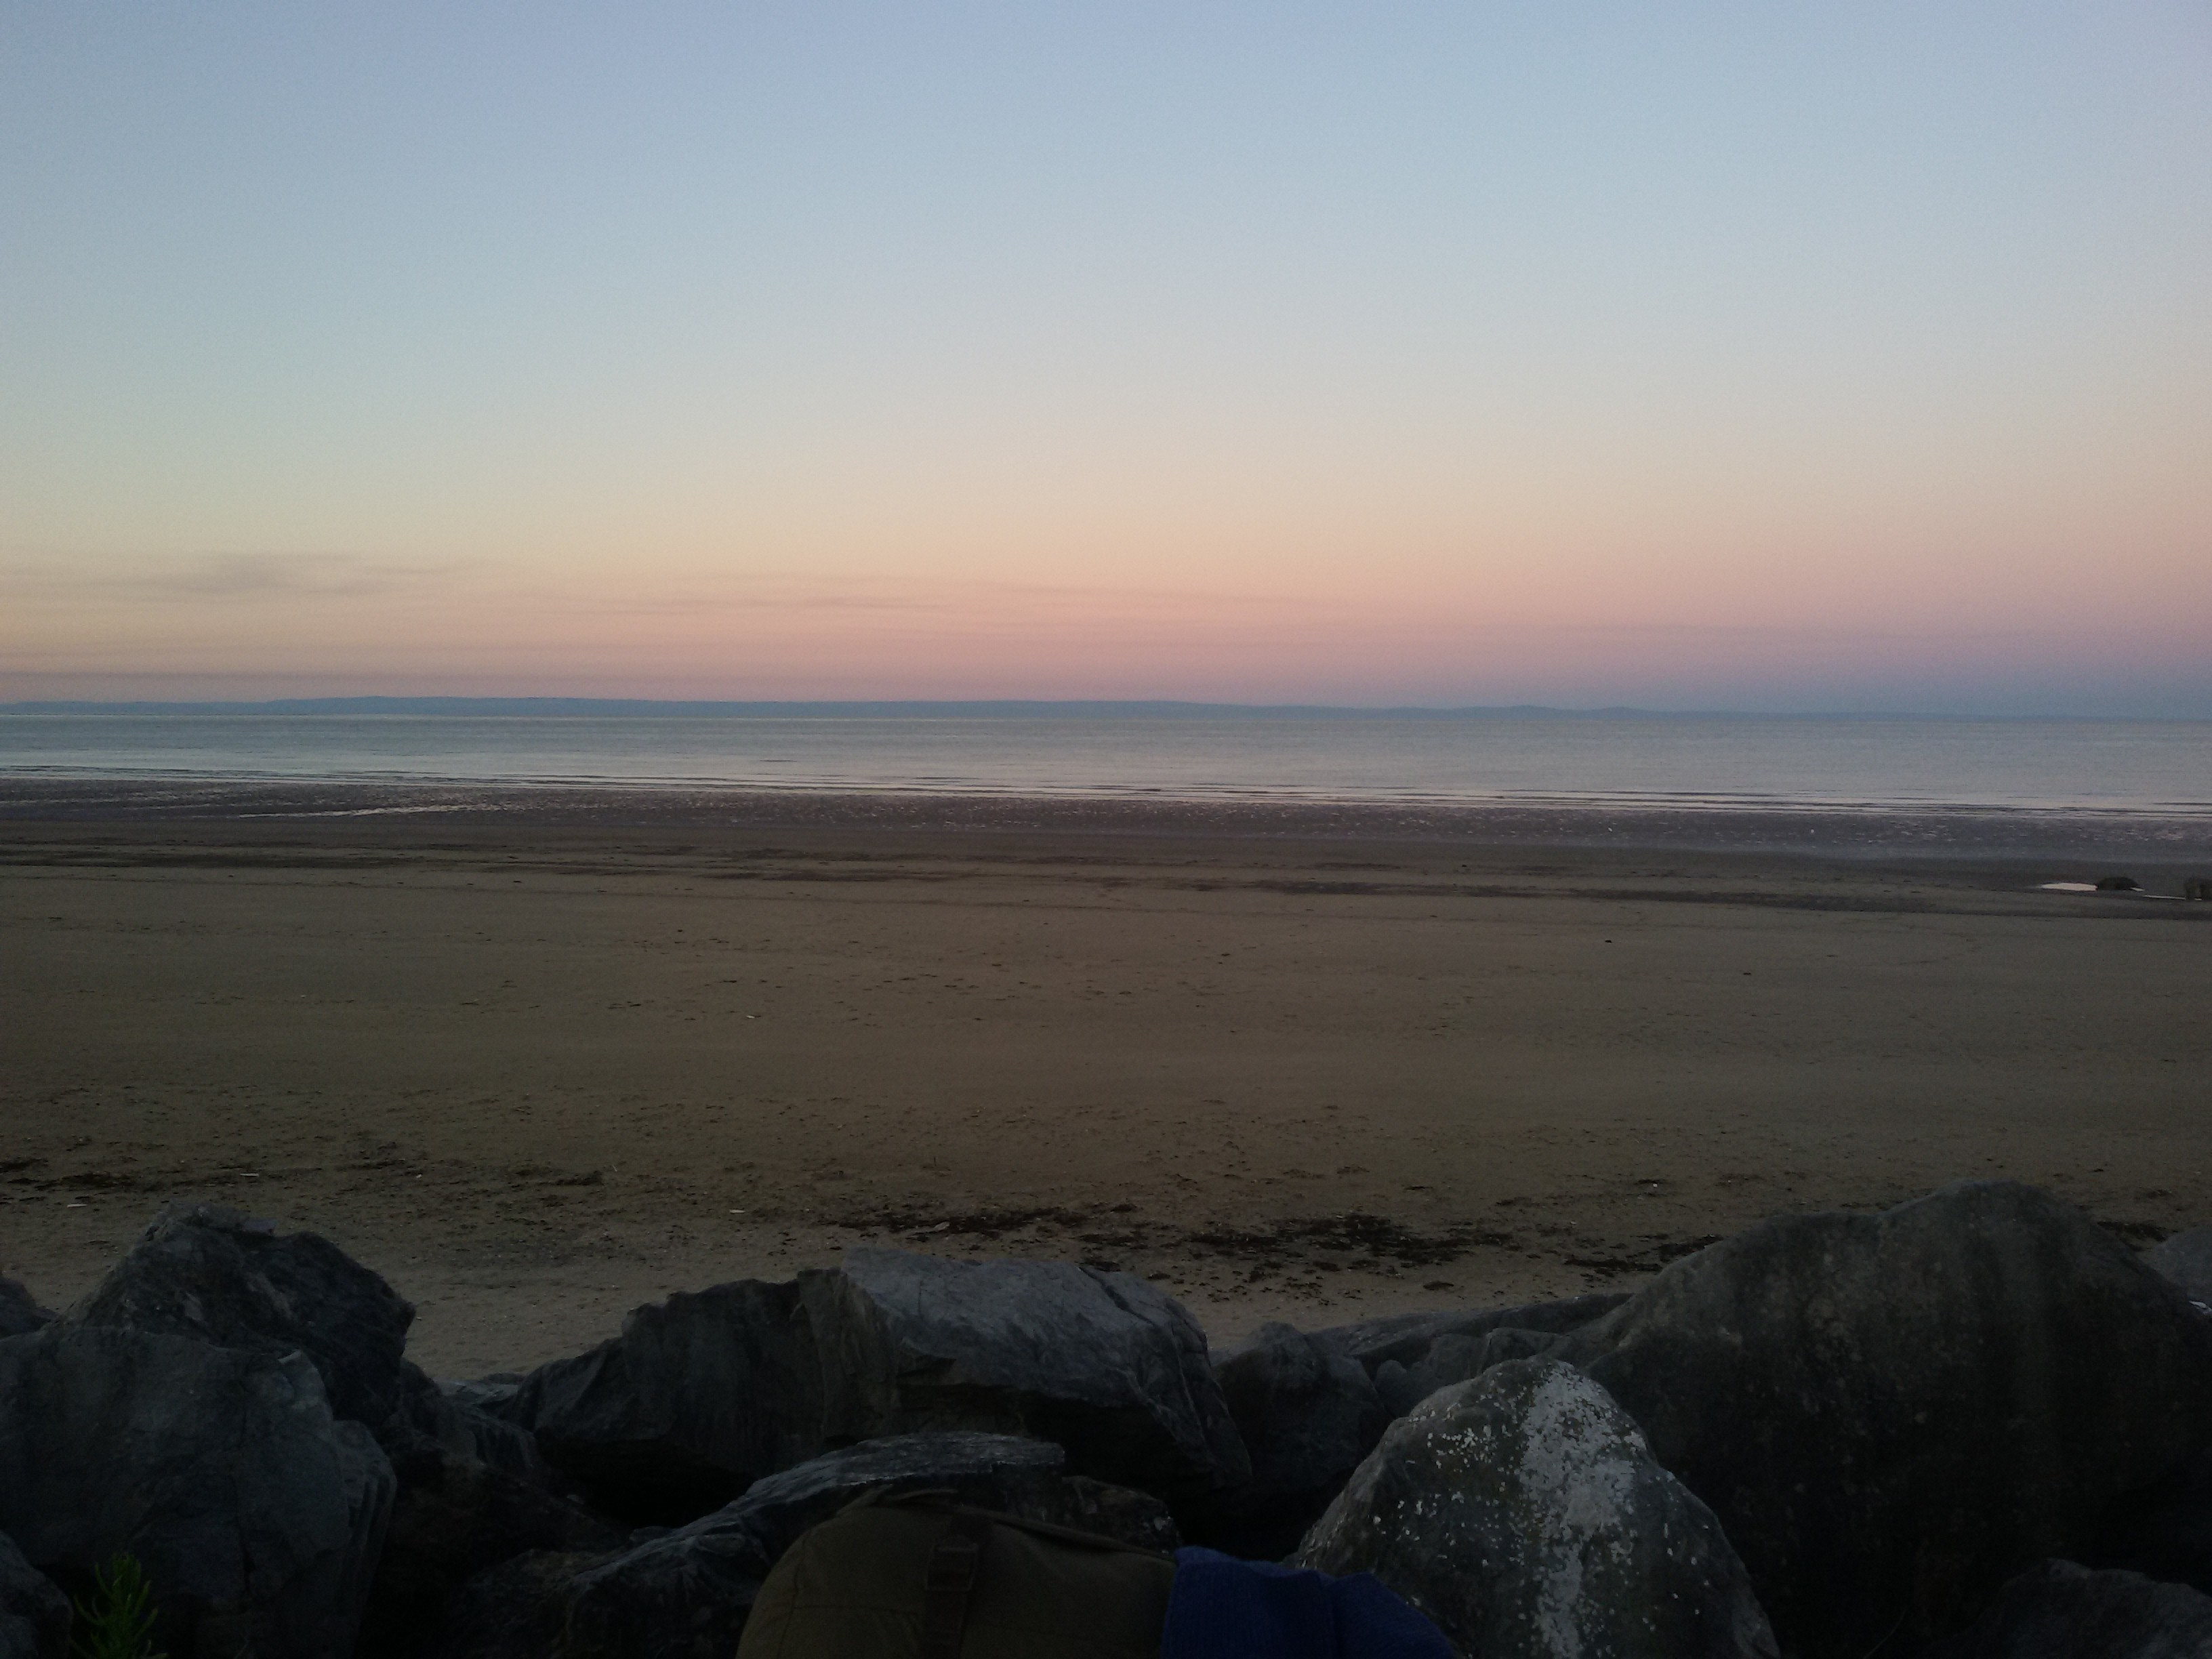
\includegraphics[width=\paperwidth]{swansea-bay}\end{minipage}}
\begin{frame}[c]
  \centering

  \bigskip
  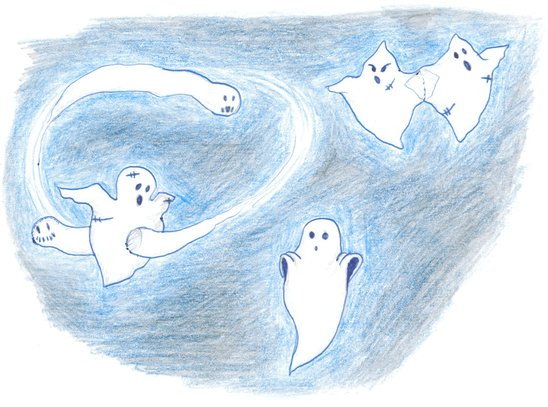
\includegraphics[height=0.32\textwidth]{phantoms}
  \bigskip
  \bigskip
  \bigskip
  \color{white}

  \begin{tikzpicture}
    \def\R{8pt}
    \node (title) {\phantom{qquad}\textcolor{white}{Maximal ideals in rings, constructively}\phantom{qquad}};
    \begin{pgfonlayer}{background}
      \draw[decorate, very thick, draw=white]
        ($(title.south west) + (\R, 0)$) arc(270:180:\R) --
        ($(title.north west) + (0, -\R)$) arc(180:90:\R) --
        ($(title.north east) + (-\R, 0)$) arc(90:0:\R) --
        ($(title.south east) + (0, \R)$) arc(0:-90:\R) --
        cycle;
    \end{pgfonlayer}
  \end{tikzpicture}

  \scriptsize
  \textit{-- an invitation --}

  \bigskip
  %(Agda formalization available)
  %\bigskip

  Computability in Europe 2022: \\
  \emph{Revolutions and Revelations in Computability} \\
  11--15 July 2022, Swansea
  \ \\
  \bigskip
  \bigskip
  \bigskip

  \begin{columns}
    \begin{column}{0.4\textwidth}
      \centering
      Ingo Blechschmidt \\
      University of Augsburg
    \end{column}
    \begin{column}{0.4\textwidth}
      \centering
      Peter Schuster \\
      University of Verona
    \end{column}
  \end{columns}
  \par
\end{frame}}

\begin{frame}{In this talk}
  \bigskip

  \begin{columns}
    \begin{column}{0.3\textwidth}
      \centering\footnotesize
      \par
      \vspace*{-1em}
      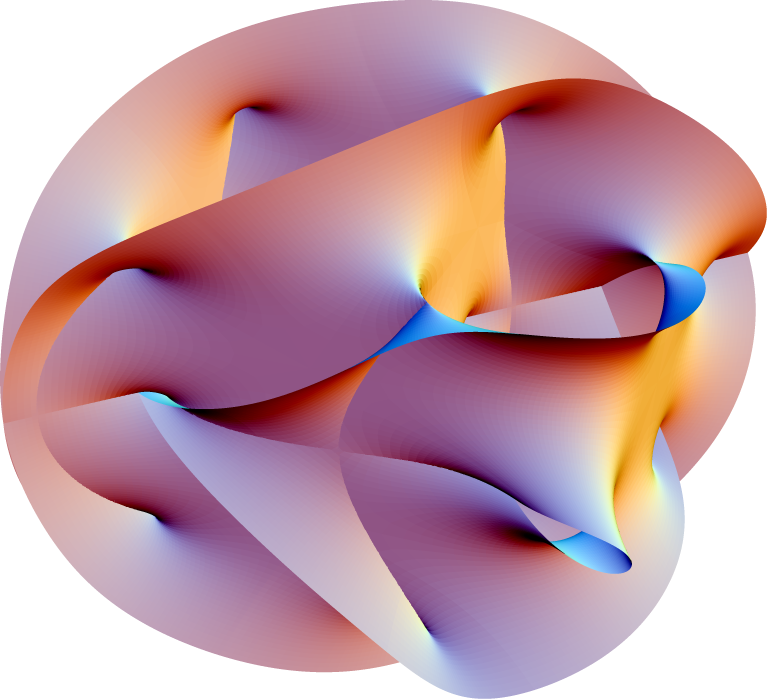
\includegraphics[height=2cm]{calabi-yau} \mbox{commutative} \\ \mbox{algebra}
    \end{column}
    \begin{column}{0.3\textheight}
      \centering\footnotesize
      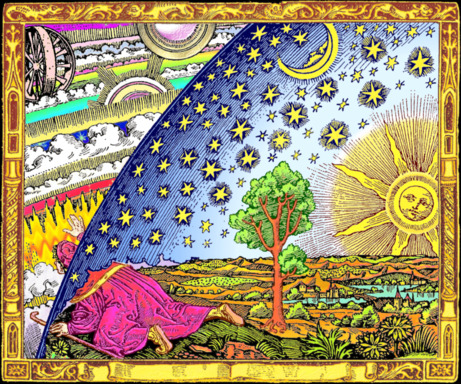
\includegraphics[height=2cm]{multiverse} \mbox{traveling} the
      \mbox{multiverse}
    \end{column}
    \begin{column}{0.3\textheight}
      \centering\footnotesize
      \par
      \vspace*{-1em}
      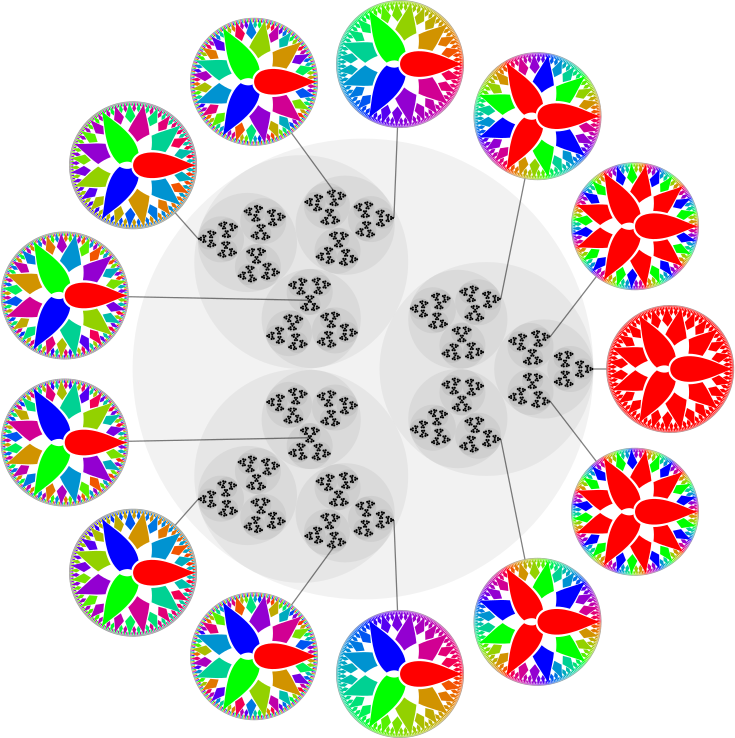
\includegraphics[height=2cm]{3-adic-numbers} \mbox{a fractal} \mbox{without points}
    \end{column}
  \end{columns}

  \medskip
  \medskip
  \medskip
  \medskip

  \begin{columns}
    \begin{column}{0.4\textwidth}
      \centering\footnotesize
      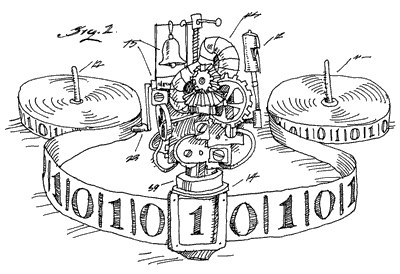
\includegraphics[height=2cm]{turing-machine} \mbox{proofs as programs}
    \end{column}
    \begin{column}{0.4\textheight}
      \centering\footnotesize
      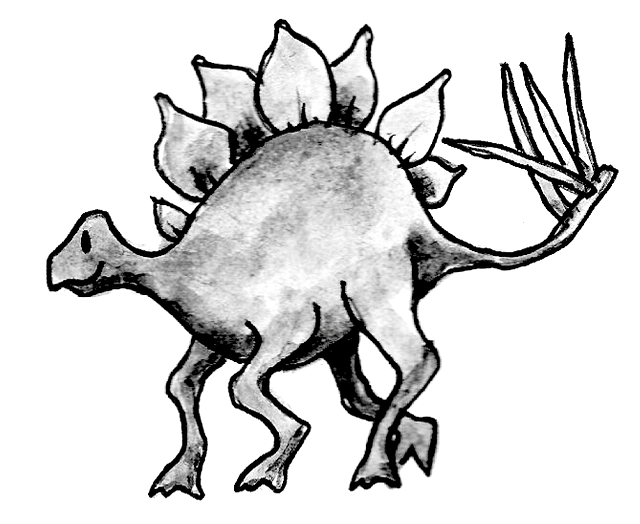
\includegraphics[height=2cm]{monad} monadic side effects
    \end{column}
  \end{columns}
\end{frame}

{\usebackgroundtemplate{\begin{minipage}{\paperwidth}\vspace*{4.95cm}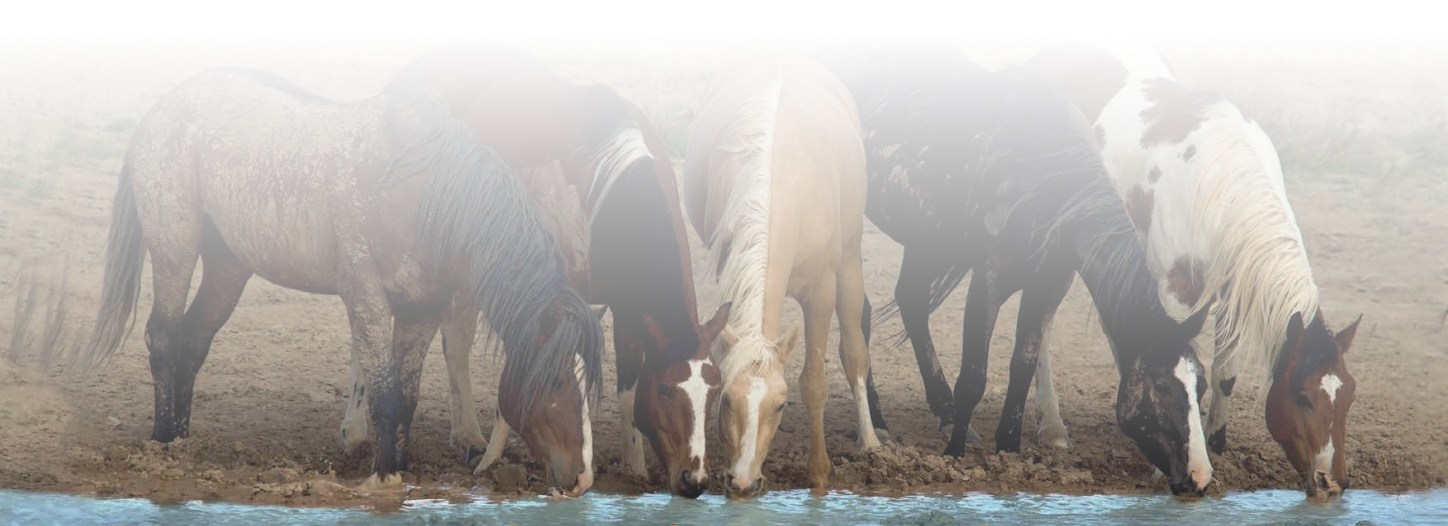
\includegraphics[width=\paperwidth]{topos-horses}\end{minipage}}
\begin{frame}{What others are saying}
  \begin{columns}
    \begin{column}{0.3\textwidth}
      \begin{tikzpicture}
        \node (inner) at (17.3mm,-20mm) {\textit{``a bad joke''}};
        \path (0,0) pic{laurel-wreath};
      \end{tikzpicture}
    \end{column}

    \begin{column}{0.3\textwidth}
      \begin{tikzpicture}
        \node (inner) at (17.5mm,-18mm) {\vbox{\small\centering\textit{``non- \\informative''}}};
        \path (0,0) pic{laurel-wreath};
      \end{tikzpicture}
    \end{column}
  \end{columns}
\end{frame}}

{\usebackgroundtemplate{\begin{minipage}{\paperwidth}\vspace*{5.95cm}
\includegraphics[width=\paperwidth]{fr1}\end{minipage}}
\begin{frame}{Transfinite methods in algebra}
  \vspace*{-1em}

  \only<1>{
    \begin{varblock}{\textwidth}{}
      \justifying
      \textbf{Theorem.}
      Let~$M$ be a surjective matrix with more rows than columns over a field.
      Then~$\lightning$.
    \end{varblock}

    \textbf{Proof.} Elementary linear algebra. \qed
  }

  \pause

  \begin{varblock}{\textwidth}{}
    \justifying
    \textbf{Theorem.}
    Let~$M$ be a surjective matrix with more rows than columns over a ring~$A$.
    Then~$1 = 0$ in~$A$.
  \end{varblock}
  \only<2>{\phantom{\textbf{Proof.} Elementary linear algebra. \qed}}%
  \pause\justify%
  \textbf{Proof.}
  \bad{Assume not.} \pause Then there is~a \bad{maximal ideal} $\mmm$. \pause
  The matrix is surjective over the field~$A/\mmm$. This is a contradiction to
  basic linear algebra. \qed

  \pause
  \textbf{Proof.}
  Write~$M = \left(\begin{smallmatrix}x\\y\end{smallmatrix}\right)$. By surjectivity,
  have~$u, v \in A$ with
  \[
    u \left(\begin{smallmatrix}x\\y\end{smallmatrix}\right) = \left(\begin{smallmatrix}1\\0\end{smallmatrix}\right)
    \quad{\text{and}}\quad
    v \left(\begin{smallmatrix}x\\y\end{smallmatrix}\right) = \left(\begin{smallmatrix}0\\1\end{smallmatrix}\right).
  \]
  Hence
  $
    1 = -\underbrace{(vy - 1)}_{=0} - vy \underbrace{(ux - 1)}_{=0} + vx
    \underbrace{(uy - 0)}_{=0} = 0
  $. \qed

  \pause
  \bigskip
  \centering
  \colorbox{white!20}{\emph{Abstract proofs should be blueprints for concrete ones.}}
\end{frame}}

\begin{frame}{The status of maximal ideals}
  \begin{itemize}
    \item[\triang] In \bad{classical mathematics}, every ring has a maximal ideal.

    \small
    -- \emph{Zorn's lemma}
    \bigskip\pause

    \normalsize
    \item[\triang] Without \bad{Zorn}, every \bad{countable} ring has a maximal ideal.

    \small
    \emph{\mbox{-- Iterative construction\only<-4>{ given
    enumeration~$x_0,x_1,\ldots$}
    [Krull 1929]\only<-4>{:}}}
    \only<-4>{\begin{align*}
      \mmm_0 &= \{ 0 \}, &
      \mmm_{n+1} &= \begin{cases}
        \mmm_n + (x_n), & \text{if $1 \not\in \mmm_n + (x_n)$}, \\
        \mmm_n, & \text{else.}
      \end{cases}
      \intertext{\visible<3->{\mbox{\emph{-- Also constructively! [Krivine
      1996], [Berardi--Valentini 2004]}}}}
      \action<3->{\mmm_0 &= \{ 0 \}, &
      \mmm_{n+1} &= \mmm_n + (\underbrace{\{ x_n \,|\, 1 \not\in \mmm_n + (x_n)
      \}}_{\text{a certain subsingleton set}})}
    \end{align*}}
    \only<5->{\mbox{\emph{-- Also constructively! [Krivine
      1996], [Berardi--Valentini 2004]}}}%
    \pause
    \pause

    \mbox{\phantom{\emph{--}} $A/\mmm$ is a residue field: noninvertible
    implies zero.}
    \bigskip

    \pause
    \pause
    \normalsize
    \item[\triang] Constructively, \neutral{every} ring has a maximal ideal in
    \mbox{\neutral{some extension of the base universe}.}

    \small
    \mbox{\emph{-- \neutral{First-order consequences} of its existence \neutral{pass
    down} to the base.}}

    \mbox{\emph{-- Obtained by applying K/B--V to the \neutral{generic surjection} $\NN
    \twoheadrightarrow A$}}
    \mbox{\emph{\phantom{--} [Joyal--Tierney 1984].}}
  \end{itemize}
\end{frame}

% \begin{document}

\begin{frame}{The generic surjection}
  Let~$A$ be a (perhaps uncountable) set.

  \begin{itemize}
    \item[\triang] Idea: Approximate the generic surjection $f : \NN
    \twoheadrightarrow A$ by \neutral{dynamically growing} partial
    functions $[x_0,\ldots,x_n]$.

    {\small
    \it
    \mbox{-- As a proof runs its course and requires that some element~$a \in A$}
    \mbox{\phantom{--} is contained in the image of~$f$, refine
    $[x_0,\ldots,x_n]$ to $[x_0,\ldots,x_n,a]$.}}

    \medskip\pause
    \item[\triang] The finite approximations serve as the \neutral{generating
    opens} of a \neutral{pointfree space}.

    {\small
    \it
    \mbox{-- There is no fact of the matter whether ``$f(0) = x \wedge
    f(1) = y$''.}

    \phantom{--} Instead, this statement has the truth value~$[x,y]$.}

    \medskip\pause
    \item[\triang]\justify Boils down to parametrizing everything by the
    current approximation and computing in the \textsf{Eventually} monad or its
    coarser cousin, the \textsf{State} monad.
  \end{itemize}
\end{frame}

\begin{frame}{Applications}
  \emph{Conceptual:}
  \begin{itemize}\small
    \item[\triang] Case study for proofs in algebra with minimal logic
    \item[\triang] New constructive proof of formal substitute for existence:

    \mbox{\emph{If the theory of maximal ideals of~$A$ is inconsistent, then~$1 =
    0$ in~$A$.}}
    \item[\triang] Strengthening of the position of maximal ideals as useful
    fictions
    \item[\triang] Reification of dynamical algebra
  \end{itemize}
  \bigskip

  \emph{Concrete:} New constructive proofs of \ldots
  \begin{itemize}\small
    \item[\triang] Krull's lemma and its corollaries
    \item[\triang] basic results of linear algebra over rings
    \item[\triang] Suslin's lemma (key to the solution of Serre's problem)
  \end{itemize}
\end{frame}

{\usebackgroundtemplate{\begin{minipage}{\paperwidth}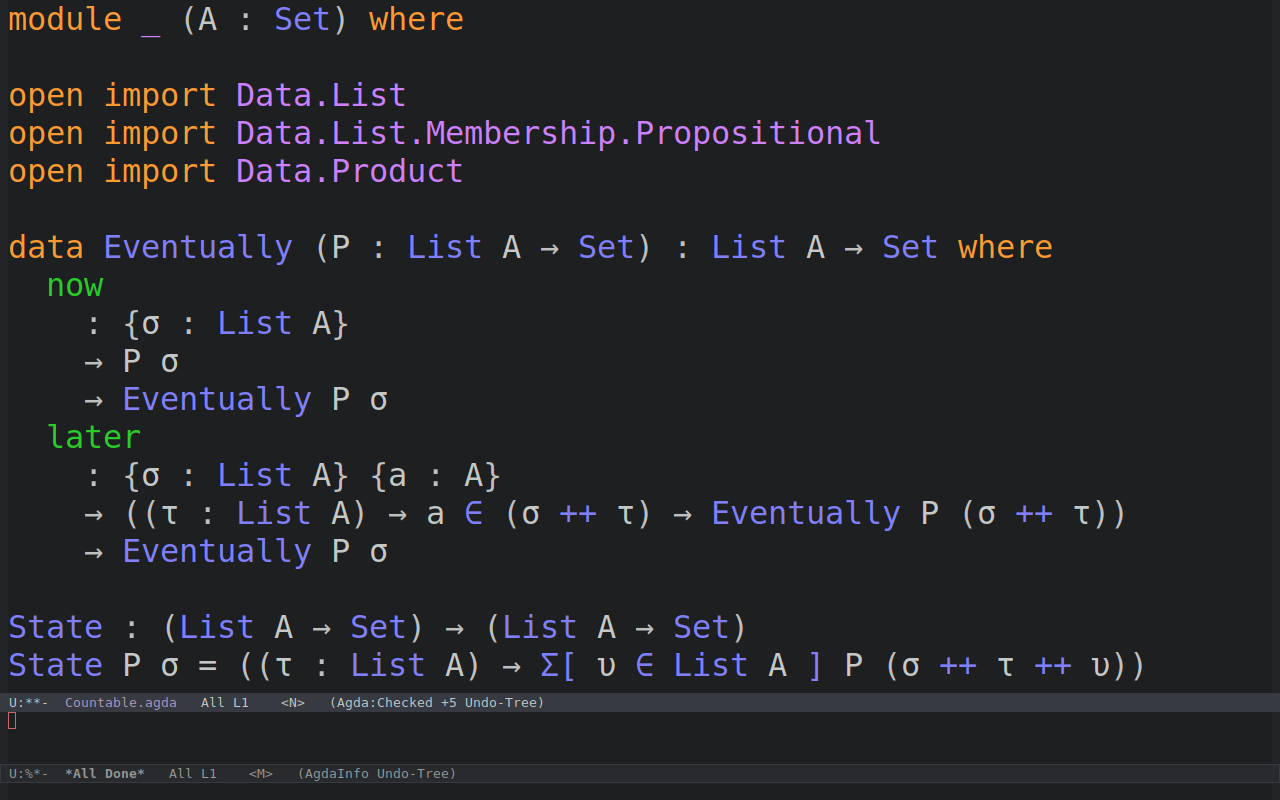
\includegraphics[width=\paperwidth]{eventually-monad}\end{minipage}}
\begin{frame}
  \vspace*{\paperheight}\vspace*{-3.5em}\centering
  \emph{Agda formalization available.}
\end{frame}}

\end{document}
